\subsection{Numerical Evaluation}\label{sec:application:cloud_file_synchronisation:numerical_evaluation}
In order to evaluate the proposed model we use the OMNeT++\footnote{\url{http://www.omnetpp.org/}} simulation framework.
To analyze the impact of the different algorithms we study the metrics introduced in \refsec{sec:application:cloud_file_synchronisation:system_model}.
We evaluate the waiting time \sojournTime until a file is retrieved at the downloading client, the relative time the mobile client stays disconnected \relativeDisconnectedTime during the synchronization process, and the number of connection \connectionCount during the synchronization process to estimate the signaling overhead.
For the \algointerval scheduling algorithm, we vary the interval length from \SI{1}{\second} to \SI{512}{\second} in powers of two.
The threshold for the \algosize algorithm is analyzed for values from \SI{1}{\mega\byte} to \SI{512}{\mega\byte} in the same manner.
The \algoimmediate algorithm is not parameterized.

In the simulated scenario, we assume a user synchronizing \(\numberOfFiles = 1000\) files from the camera to the downloading client.
For each parameter set we perform \(100\) repetitions.

\subsubsection*{Waiting Time}\label{sec:application:cloud_file_synchronisation:numerical_evaluation:waiting_time}
First, we analyze the waiting time \sojournTime required to transfer a picture from the camera to the wire-lined download client for the different scheduling algorithms and different parameter sets.
The mean waiting times and the corresponding \SI{95}{\percent} confidence intervals are shown in \reffig{fig:application:cloud_file_synchronisation:numerical_evaluation:waiting_time:waiting_time}.
For most of the derived mean values, the confidence intervals are not visible due to their small size.

\begin{figure}
	\begin{subfigure}[b]{\textwidth}
	\centering
	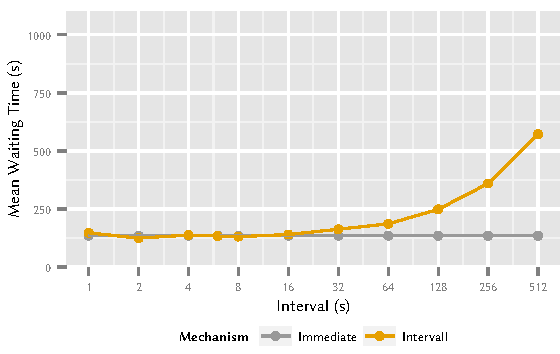
\includegraphics{application/cloud_file_synchronization/numerical_evaluation/figures/interval_delay}
	\caption{Algorithm \algointerval for different interval lengths}\label{fig:application:cloud_file_synchronisation:numerical_evaluation:waiting_time:waiting_time:interval}
	\end{subfigure} 
	\begin{subfigure}[b]{\textwidth}
	\centering
	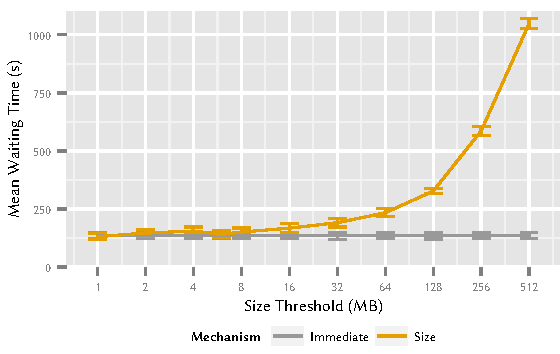
\includegraphics{application/cloud_file_synchronization/numerical_evaluation/figures/size_delay}
	\caption{Algorithm \algosize for threshold sizes}\label{fig:application:cloud_file_synchronisation:numerical_evaluation:waiting_time:waiting_time:size}
	\end{subfigure}

	\caption{Comparison of algorithms with regard to waiting time \sojournTime}\label{fig:application:cloud_file_synchronisation:numerical_evaluation:waiting_time:waiting_time}
\end{figure}

\reffig{fig:application:cloud_file_synchronisation:numerical_evaluation:waiting_time:waiting_time:interval} shows the results for the \algointerval algorithm, \reffig{fig:application:cloud_file_synchronisation:numerical_evaluation:waiting_time:waiting_time:size} shows the results for the \algosize mechanisms. 
In \reffig{fig:application:cloud_file_synchronisation:numerical_evaluation:waiting_time:waiting_time:interval} the x-axes shows the length of the interval in \si{\second} between sending newly added files, in \reffig{fig:application:cloud_file_synchronisation:numerical_evaluation:waiting_time:waiting_time:size} the axis shows the required cumulated size in \si{\mega\byte} of new files before an upload is triggered.
The y-axes in both figures show the mean waiting time \sojournTime in \si{\second}.
The result of the \algoimmediate algorithm is added in both figures as a reference.
Note, the waiting time for this algorithms is independent of the parameters used for the other two algorithms, as files are always uploaded immediately after they have been copied to the \dropbox folder.

\reffig{fig:application:cloud_file_synchronisation:numerical_evaluation:waiting_time:waiting_time:interval} shows that the waiting time dependents on the inter-send interval of the \algointerval algorithm. 
For inter-send intervals smaller than \SI{8}{\second}, the waiting times do not differ significantly from the waiting times obtained by the \algoimmediate algorithm.
This can be explained by the average file size of \SI{3.5}{\mega\byte} of the images and the assumed average Bluetooth transmission rate of \SI{0.5}{\mega\bit\per\second}, which results in an average inter arrival time of \SI{7}{\second}.
For inter-send interval less than \SI{7}{\second}, there is almost always an image in the upload queue so that the algorithm performs similar to the \algoimmediate strategy. 
For inter-send intervals larger than \SI{7}{\second}, the average waiting time increases for the \algointerval algorithm.
Here, the files are already preprocessed and accumulate in the uploading queue until the next batch upload starts resulting in an increased mean waiting time.
For very large values of the inter-send interval, the waiting time is dominated by the interval length.
This mean that the mobile client's waiting time before starting the upload is much longer that the upload duration of the images.
Thus, the mean waiting time converges to the interval length for extreme values.

\reffig{fig:application:cloud_file_synchronisation:numerical_evaluation:waiting_time:waiting_time:size} depicts the waiting time for the \algosize algorithms for different trigger file sizes.
We observer that for values smaller than the average image file size of \SI{3.5}{\mega\byte}, the \algosize algorithms performs similar to the \algoimmediate algorithms.
In this case the \algosize algorithms also triggers an upload for almost each file and  shows the same behaviour as the \algoimmediate algorithm.
For trigger threshold smaller than \SI{16}{\mega\byte}, the performance of the \algosize algorithms is only slightly worse than the reference mechanism.
Here, only a few files are required to trigger the upload process and the additional delay introduced by waiting is negligible.
For larger trigger threshold, the mean waiting time increases significantly.

\subsubsection*{Relative Disconnection Time}\label{sec:application:cloud_file_synchronisation:numerical_evaluation:relative_disconnection_time}

Besides a fast synchronization, the users also demand a long battery life time of the mobile device.
Besides the display, the RF interface used to establish Internet connection is one of the main energy consumers.
In order to analyse the energy savings of the different algorithms, we evaluate the relative disconnected time  \relativeDisconnectedTime during the synchronization process.
Therefore, we consider the time between the sending of the first and the last image of the mobile client and calculate the percentage during which no Internet connection is established.
The mean relative disconnected times including the \SI{95}{\percent} confidence intervals are depicted in \reffig{fig:application:cloud_file_synchronisation:numerical_evaluation:disconnected:disconnected}. 

\begin{figure}
	\begin{subfigure}[b]{\textwidth}
	\centering
	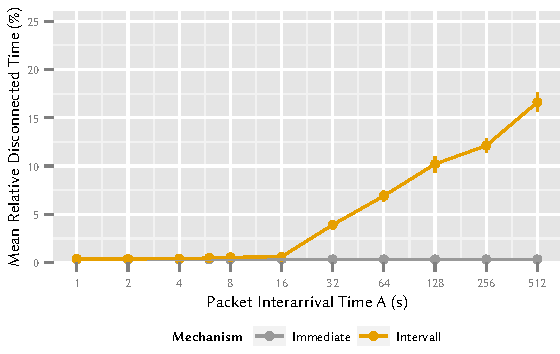
\includegraphics{application/cloud_file_synchronization/numerical_evaluation/figures/interval_disconnected}
	\caption{Algorithm \algointerval for different interval lengths}\label{fig:application:cloud_file_synchronisation:numerical_evaluation:disconnected:disconnected:interval}
	\end{subfigure} 
	\begin{subfigure}[b]{\textwidth}
	\centering
	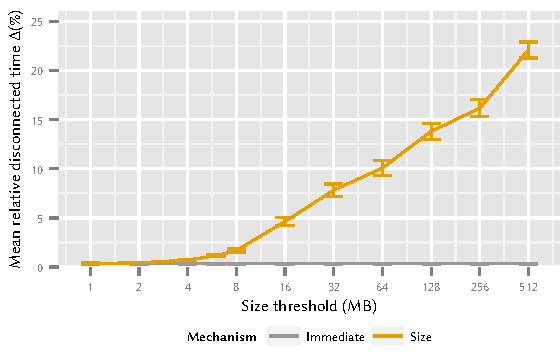
\includegraphics{application/cloud_file_synchronization/numerical_evaluation/figures/size_disconnected}
	\caption{Algorithm \algosize for threshold sizes}\label{fig:application:cloud_file_synchronisation:numerical_evaluation:disconnected:disconnected:size}
	\end{subfigure}

	\caption{Comparison of algorithms with regard to relative disconnected time relativeDisconnectedTime}\label{fig:application:cloud_file_synchronisation:numerical_evaluation:disconnected:disconnected}
\end{figure}

\reffig{fig:application:cloud_file_synchronisation:numerical_evaluation:disconnected:disconnected:interval} depicts the relative disconnected time \relativeDisconnectedTime on the y-axis, on the x-axis the inter-sending interval in \si{\second} for the \algointerval algorithm. 
\reffig{fig:application:cloud_file_synchronisation:numerical_evaluation:disconnected:disconnected:size} also depicts the relative disconnected time on the y-axis, on the x-axis the sending threshold in \si{\mega\byte} for the \algosize algorithm. 
Both figures include the \algoimmediate algorithm as a reference.

We first study \reffig{fig:application:cloud_file_synchronisation:numerical_evaluation:disconnected:disconnected:interval}.
Similar to \reffig{fig:application:cloud_file_synchronisation:numerical_evaluation:waiting_time:waiting_time:interval}, we observe no significant differences between the \algointerval and \algoimmediate algorithm for inter-send intervals smaller than \SI{8}{\second}, as both algorithms show the same behaviour here.
For values larger than \SI{8}{\second}, the \algointerval algorithm starts sending files in batches and no longer on a per file base.
However, still no clear effect is visible, because the inter-sending interval and the mean image inter-arrival time of files is still smaller than the disconnection timeout of \SI{11}{\second}.
This results in an almost permanent Internet connection similar to the \algoimmediate algorithm.
For inter-send interval above \SI{16}{\second}, the \algointerval algorithm starts saving connection time and the relative disconnected time increases, resulting in additional energy savings.

\reffig{fig:application:cloud_file_synchronisation:numerical_evaluation:disconnected:disconnected:size} shows the relative disconnected time for variable thresholds for the \algosize algorithm.
We see again that the \algosize and \algoimmediate algorithms do not differ for thresholds smaller than \SI{4}{\mega\byte}, similar to the results in \reffig{fig:application:cloud_file_synchronisation:numerical_evaluation:waiting_time:waiting_time:size}.
Afterwards, we observe an increase in saved connection time for larger thresholds, because here files are sent in batches and the mobile client disconnects between the sending intervals, again enabling energy saving potential for the mobile network client.

\subsubsection*{Connection Count}\label{sec:application:cloud_file_synchronisation:numerical_evaluation:connection_count}

After considering the requirements of the end-user, we have a closer look at the requirements of the mobile network operators.
The network operator is mainly interested in minimizing the signaling overhead introduce by connection establishment.
Therefore, a minimization of the number of connections during the synchronization process is desired.
\reffig{fig:application:cloud_file_synchronisation:numerical_evaluation:connection:connection} depicts the average number of connections \connectionCount established during the synchronization process, including the 95\% confidence intervals.
The number of connections is shown on the y-axis, the x-axis in \reffig{fig:application:cloud_file_synchronisation:numerical_evaluation:connection:connection:interval} shows the inter-send interval of the \algointerval algorithms, the x-axis in \reffig{fig:application:cloud_file_synchronisation:numerical_evaluation:connection:connection:size} shows the \algosize algorithm threshold.

\begin{figure}
	\begin{subfigure}[b]{\textwidth}
	\centering
	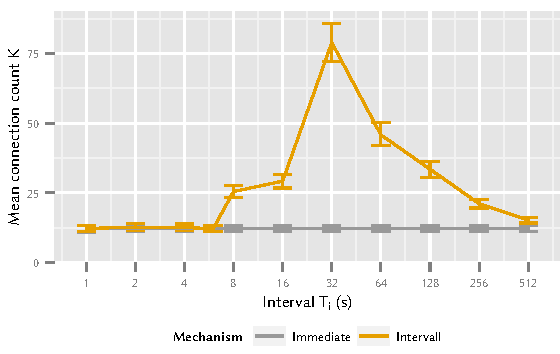
\includegraphics{application/cloud_file_synchronization/numerical_evaluation/figures/interval_connection}
	\caption{Algorithm \algointerval for different interval lengths}\label{fig:application:cloud_file_synchronisation:numerical_evaluation:connection:connection:interval}
	\end{subfigure} 
	\begin{subfigure}[b]{\textwidth}
	\centering
	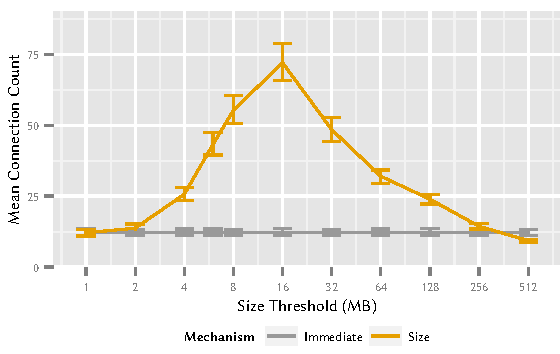
\includegraphics{application/cloud_file_synchronization/numerical_evaluation/figures/size_connection}
	\caption{Algorithm \algosize for threshold sizes}\label{fig:application:cloud_file_synchronisation:numerical_evaluation:connection:connection:size}
	\end{subfigure}

	\caption{Comparison of Algorithms with Regard to Connection Count \connectionCount}\label{fig:application:cloud_file_synchronisation:numerical_evaluation:connection:connection}
\end{figure}

We observer a similar behavior as in the previous evaluations, the average number of connection for the \algointerval and the \algoimmediate algorithms is the same in \reffig{fig:application:cloud_file_synchronisation:numerical_evaluation:connection:connection:interval}, if the inter-send intervals are smaller then \SI{4}{\second}.
With increasing inter-send intervals the connection count also increases and reaches a maximum for an interval length of \SI{32}{\second}.

%TODO: check SI containing variables
In order to explain this behaviour we make the following considerations.
The maximum amount of data \(s_x\) which can be send from the camera to the mobile client during an inter-send interval of length \(x\si{\second}\) is given by 
\[s_x=\panTransferRate \cdot x\si{\second} = x \cdot \SI{1/2}{\mega\byte}.\]
The average time \(t_x\) to upload \(s_x\) can now be calculated as 
\[t_x = \nicefrac{s_x}{E\left[\uploadbandwidth\right]} = x\SI{0.5 / 8.0}{\second} = x\SI{1 / 16}{\second}.\]
For inter-send intervals between \SI{8}{\second} and \SI{32}{\second}, \(t_x\) results in \SI{0.5}{\second}, \SI{1}{\second}, and \SI{2}{\second} respectively.
Considering the disconnection time out of \SI{11}{\second}, we can see that a disconnect is likely for interval lengths of \SI{16}{\second} and \SI{32}{\second}.
In order to explain the increased number of connections for an inter-send interval of \SI{8}{\second}, we also have to consider the average image file size of \SI{3.5}{\mega\byte}.
Within \SI{8}{\second}, a maximum  of \(s_x = \SI{4}{\mega\byte}\) can be transferred from the camera to the mobile client.
Therefore, it is likely that it takes two interval lengths, respectively \SI{16}{\second}, to transfer the image.
This explains the similar behaviour of the \algointerval algorithm for inter-send intervals of \SI{8}{\second} and \SI{16}{\second} with regard to the connection count.

For inter-send intervals larger then \SI{32}{\second}, the connection count decreases again.
To explain this effect, we have to consider the maximum number of file batches transferred during the synchronization process.
If every file is transferred individually \(1000\) connections would be required, if all files are transferred in one single batch, only one connection would be established during the synchronization process.
Depending on the chosen inter-send intervals, the average sizes of the batches varies, as larger intervals result in larger batches.
The overall number of batches is limited, because we only consider a finite amount of \(1000\) images.
Consequently, the maximum number of connections is limited, too.
However, this comes only into effect if large batch are used during the synchronization process.


In \reffig{fig:application:cloud_file_synchronisation:numerical_evaluation:connection:connection:size} we can observe similar behaviours of the \algosize algorithm as for the \algointerval algorithm in \reffig{fig:application:cloud_file_synchronisation:numerical_evaluation:connection:connection:interval}.
For small thresholds, the \algosize and the \algoimmediate algorithm result in the same number of connections.
With increasing sending thresholds, the number of disconnects and re-connections increases, as it takes longer to accumulate the required amount of new data at the mobile client.
The maximum average connection count is reached when using a \SI{16}{\mega\byte} threshold, which corresponds to \(s_x\) for an inter-sending interval of \SI{32}{\second}.
For larger thresholds, the maximum number of batches is the limiting factor for the connection count.
This can especially be observed for very large thresholds.
Considering a threshold of \SI{128}{\mega\byte}, we can assume that almost each batch is transferred in an individual connection, as it takes $\nicefrac{\SI{128}{\mega\byte}}{\panTransferRate} = \SI{248}{\second}$ to transfer the require data from the camera to the mobile client, but only \(\nicefrac{\SI{128}{\mega\byte}}{E\left[\uploadbandwidth\right]} = \SI{16}{\second}\) on average to upload the data from the mobile client to the cloud.
Consequently, the transferred file size can be estimated as the product of sending threshold and number of connections \(\SI{128}{\mega\byte} \cdot 25 = \SI{3.2}{\giga\byte}\), which approximately matches the product of number of considered files and the average file size.

\subsubsection*{Mechanism Comparison}\label{sec:application:cloud_file_synchronisation:numerical_evaluation:mechanism_comparison}
\subsubsection*{Trade-off Analysis}\label{sec:application:cloud_file_synchronisation:numerical_evaluation:trade_off_analysis}